\documentclass[11pt,a4paper]{article}

\usepackage[T1]{fontenc}
\usepackage[utf8]{inputenc}
\usepackage[margin=2.4cm]{geometry}
\usepackage{graphicx}
\usepackage{booktabs}
\usepackage{amsmath,amssymb}
\usepackage{xcolor}
\usepackage{tcolorbox}
\usepackage{caption}
\usepackage{float}
\usepackage{enumitem}
\usepackage{longtable}
\usepackage[hidelinks]{hyperref}

\definecolor{kuetblue}{RGB}{20,60,110}
\definecolor{softgrey}{RGB}{245,245,247}

\captionsetup{font=small,labelfont=bf}
\setlist{itemsep=2pt,parsep=0pt,topsep=3pt}

\newtcolorbox{keybox}[1]{colback=softgrey,colframe=kuetblue,
  fonttitle=\bfseries,title=#1,boxrule=0.6pt,left=6pt,right=6pt,top=4pt,bottom=4pt}

\title{\vspace{-1.2cm}\textbf{Predicting University Website Quality\\from Measurable Page Attributes}\\[4pt]
\large A Two-Track Labelling Design that Avoids Circular Evaluation}
\date{}

\begin{document}

%========================================================= TITLE PAGE
\begin{titlepage}
\centering
\vspace*{1.2cm}

{\Large\bfseries Khulna University of Engineering \& Technology}\\[3pt]
{\large Department of Computer Science and Engineering}\\[1.6cm]

\rule{\textwidth}{1pt}\\[10pt]
{\LARGE\bfseries Predicting University Website Quality\\[6pt] from Measurable Page Attributes}\\[10pt]
{\large A Two-Track Labelling Design that Avoids Circular Evaluation}\\[8pt]
\rule{\textwidth}{1pt}\\[1.4cm]

{\large\bfseries Course:} Machine Learning Laboratory\\[2pt]
{\large\bfseries Course Code:} CSE 4112\\[1.6cm]

{\large\bfseries Submitted By}\\[8pt]
\begin{tabular}{ll}
\toprule
\textbf{Name} & \textbf{Roll} \\
\midrule
Faisal Ahmed          & 2107061 \\
Al Shariar Hossain    & 2107066 \\
Md. Rubayet Nabil     & 2107073 \\
Khadimul Islam Mahi   & 2107076 \\
Abhijeet Deb Nath     & 2107083 \\
Afifa Sultana Offa    & 2107087 \\
\bottomrule
\end{tabular}\\[1.4cm]

{\large\bfseries Submitted To}\\[6pt]
\fbox{\parbox{0.55\textwidth}{\centering\vspace{3pt}
\textcolor{red}{\textbf{[ SUPERVISOR NAME AND DESIGNATION ]}}\\[2pt]
\small Department of Computer Science and Engineering\\
Khulna University of Engineering \& Technology\vspace{3pt}}}\\[4pt]
{\footnotesize\itshape The Lab~3 report supplied for reference contains no supervisor name;\\
please fill this box in before submitting.}\\[1.2cm]

\vfill
{\large Date of Submission: \today}
\end{titlepage}

%========================================================= ABSTRACT
\section*{Abstract}
\addcontentsline{toc}{section}{Abstract}

We build a model that reads 78 measurable attributes of a university landing page and returns
a $0$--$100$ website--quality score, then use it to rank 1{,}226 university websites globally.
The central difficulty is not modelling but \emph{labelling}: the dataset ships without a
target column, and the obvious fix --- inventing a weighted formula over the features and
training a model to predict it --- produces a near-perfect $R^2$ that measures nothing. We
therefore separate the two roles. Track~A is an explicit, auditable rubric that serves as the
\emph{baseline}; Track~B is a set of 900 blind pairwise judgments over 200 anonymised profile
cards, converted to a latent score by the Bradley--Terry model, which serves as the
\emph{target}. Because Track~B is not a closed-form function of the features, Spearman$(A,B)$
becomes a real empirical result rather than an identity.

Our labelling was performed twice, and the difference between the two passes is the paper's
main methodological finding. The first pass produced a label dominated by \emph{alt-text
coverage} --- an attribute no site visitor can perceive --- because the profile cards
advertised it as a headline number, and it was further corrupted by median imputation that
described 469 sites with no dated notice at all as having ``posted yesterday''. After fixing
the missing-value policy and re-framing the judging question around what a prospective
applicant actually needs, all 900 pairs were re-judged. Alt-text citations fell from
$37.6\%$ to $0\%$, admission-task content rose from $38.1\%$ to $73.1\%$, and $16.4\%$ of
winners changed --- the signature of a genuine criterion change rather than noise.
Self-consistency on swapped repeat pairs rose to $96.7\%$.

On the corrected label, a LightGBM regressor reaches Spearman $\rho = 0.922$ ($R^2 = 0.818$,
MAE $= 9.0$ points) on a 40-university test set held out from every fitting and tuning
decision, against $\rho = 0.810$ for the transparent rubric it must beat. Leave-one-region-out
validation gives $\rho = 0.844$, confirming the model learned quality rather than geography.

%========================================================= 1
\section{Introduction and Problem Statement}

\subsection{What the system does}

\begin{center}
\begin{tabular}{c@{\hspace{6pt}}c@{\hspace{6pt}}c@{\hspace{6pt}}c@{\hspace{6pt}}c}
\fbox{\parbox{3.0cm}{\centering\small\textbf{INPUT}\\[2pt]78 measured\\attributes of one\\landing page}}
& $\longrightarrow$ &
\fbox{\parbox{3.0cm}{\centering\small\textbf{MODEL}\\[2pt]LightGBM\\regressor}}
& $\longrightarrow$ &
\fbox{\parbox{3.6cm}{\centering\small\textbf{OUTPUT}\\[2pt]quality score $0$--$100$\\+ grade + global,\\regional, country rank}}
\end{tabular}
\end{center}

\noindent Concretely, given a row such as ``lists programmes: yes; departments page: yes;
admissions policy: no; latest notice: 30 days old; menu: 6 items; contrast 13.3:1; mobile
score 75'', the system returns \textbf{85.9 / 100, grade A+, global rank 31 of 1226}. Higher
is better throughout: the best sites score near 92, the worst near 0.

\subsection{Why this is not a trivial regression}

A quality score has to come from somewhere. The tempting shortcut is to define
$y = 0.5\,c + 0.3\,u + 0.2\,s$ over content, usability and speed features, then train a model
to predict $y$. This reports $R^2 \approx 0.98$ and proves only that a learner can re-derive
our own arithmetic. Biyyapu et al.~(2023) published exactly this design and reported $98.2\%$
accuracy for predicting a lookup table from its own inputs. Avoiding that circularity is the
organising constraint of this project, and it is why roughly half the work reported here is
about the label rather than the model.

\subsection{Contributions}

\begin{enumerate}
\item A \textbf{two-track labelling design} that keeps the auditable formula as a baseline and
      uses independent holistic judgment as the target, making the rubric--label agreement a
      measurable result instead of a tautology.
\item A documented \textbf{label failure and repair}. We show quantitatively that our first
      label measured the wrong construct, diagnose both causes, repair them, and re-judge all
      900 pairs so that the two passes form a controlled comparison.
\item An explicit \textbf{null-is-not-zero missing-value policy}, motivated by a concrete case
      in which median imputation inverted the meaning of the strongest freshness feature.
\item A global ranking of 1{,}226 university websites with SHAP-based explanations, a
      per-university improvement report, leave-one-region-out fairness analysis, and a
      quantified statement of what the ranking cannot see.
\end{enumerate}

%========================================================= 2
\section{Dataset and Audit}

The raw dataset contains 1{,}230 university landing pages described by 69 attributes,
organised into 11 blocks (B1 header/navigation, B2 rankings/recognition, B3 notices/updates,
B4 events/media, B5 page content, B6 footer, B7 visual design, B8 service interaction,
B9 technical performance, B10 SEO metadata, B11 accessibility). Every finding below was
re-derived in code in notebook \texttt{01\_audit} rather than assumed.

\begin{table}[H]\centering\small
\caption{Audit findings and the action taken. Nothing was silently corrected.}
\begin{tabular}{p{5.6cm}p{3.0cm}p{6.2cm}}
\toprule
\textbf{Finding} & \textbf{Scale} & \textbf{Action} \\
\midrule
Prestige columns almost entirely null & \texttt{a10} 99.35\% null, \texttt{a08} 94.96\% null & Dropped: unusable \emph{and} a leakage risk \\
Exact duplicate column & \texttt{load\_time\_s} $\equiv$ \texttt{a62} & One dropped \\
Constant / empty columns & 3 columns & Dropped \\
Duplicate domains & 4 pairs (8 rows) & Merged to 1{,}226 rows; load time set to the pair median; mislabelled country fixed \\
Notice dates after the crawl date & 285 of 759 & Censored to the crawl date; flag retained \\
Notice flags contradict the dates & 382 + 156 rows & Reconciled into an ordinal \texttt{notice\_evidence} $\in \{0,1,2,3\}$ \\
Event flags contradict the counts & 327 + 158 rows & Reconciled into \texttt{event\_evidence} \\
Collector $\perp$ region is 1:1 & 6 collectors, 6 regions & \textbf{Unresolvable}; reported as a limitation \\
Load time varies by region & median 8.07\,s to 12.94\,s & Region $z$-scored; every ranking produced with and without it \\
Country field mixes levels & 10 bucket labels, 170 rows & Country ranking restricted to the 19 real countries with $\geq 20$ universities \\
\bottomrule
\end{tabular}
\end{table}

\subsection{The missing-value policy: null is not zero, and not the median either}

\begin{keybox}{The most consequential decision in the pipeline}
The median of \texttt{notice\_recency\_days} is \textbf{1 day}. Median-imputing it would tell
every downstream consumer that the \textbf{469 universities with no dated notice anywhere on
their site posted something yesterday} --- handing the strongest freshness signal in the
dataset to exactly the sites that earned it least. Absence was being read as average when it
means \emph{absent}.
\end{keybox}

\noindent Where absence has a known direction, the feature is filled at the worst defensible
value instead, and the rule is written to \texttt{missing\_value\_policy.json}:

\begin{table}[H]\centering\small
\begin{tabular}{lrrl}
\toprule
\textbf{Feature} & \textbf{Rows filled} & \textbf{Fill} & \textbf{Meaning of absence} \\
\midrule
\texttt{notice\_recency\_days} & 469 & 3650 d & no dated notice exists at all \\
\texttt{a72\_alt\_text\_pct}   & 4   & 0\%    & no image carries a text alternative \\
\texttt{a53\_contrast\_ratio}  & 1   & 1.0:1  & no readable text block was found \\
\bottomrule
\end{tabular}
\end{table}

\noindent Companion \texttt{*\_missing} indicator columns are computed \emph{before} the fill,
so ``this was never measured'' remains recoverable as a separate fact.

%========================================================= 3
\section{The Labelling Design}

\subsection{Track A --- the transparent rubric (baseline, not target)}

Track~A is a rubric written and frozen \emph{before} any score was computed. It applies:

\begin{itemize}
\item \textbf{Gates} that cap the achievable score regardless of everything else: no primary
      navigation caps at 45; no HTTPS caps at 60.
\item \textbf{Six tiers}, heaviest first: can-I-do-the-task content; is-this-alive evidence;
      depth of service; accessibility and technical; polish; and self-promotion (ranking
      badges, trust seals, testimonials) at near-zero weight.
\item \textbf{Non-linear response curves} that a correlation matrix cannot produce --- an
      inverted-U on menu size (0--2 items is broken, 5--9 ideal, 15+ cluttered), diminishing
      returns on statistic counts, a plateau on contrast at 7:1 (WCAG AAA, since 21:1 is not
      better than 12:1), and half credit for undated notices.
\item \textbf{Five personas} (domestic applicant, international applicant, accessibility
      specialist, researcher, literature-aligned), averaged into \texttt{trackA\_consensus},
      with the between-persona standard deviation retained as a per-university uncertainty.
\end{itemize}

Track~A is a deterministic function of the features. A model predicting it would score
$R^2 \approx 0.98$ and demonstrate nothing, so it is used strictly as \textbf{the baseline the
learned model must beat}.

\subsection{Track B --- blind pairwise judgment (the target)}

200 universities were sampled, stratified by region and across the full Track~A range. Each
was rendered as an \textbf{anonymised profile card} carrying no name, country, region, URL,
collector or Track~A score --- blinding is what prevents prestige and rubric anchoring from
leaking into the label. Cards were presented in 900 pairs: 500 random (for graph connectivity
and wide gaps), 340 matched within $\pm 5$ Track~A points (the hard, informative cases), and
60 repeats re-presented later with the sides swapped. Left/right position was randomised.

Judgments were then fitted with the \textbf{Bradley--Terry} model,
\[
P(i \text{ beats } j) = \sigma(\beta_i - \beta_j),
\]
estimated by $L_2$-regularised logistic regression on a $\pm 1$ design matrix with no
intercept, with bootstrap confidence intervals on each $\beta_i$. The resulting latent
strength $\beta$ is the supervised target \texttt{trackB\_bt\_score}.

%========================================================= 4
\section{The Relabelling: A Documented Repair}

Our first labelling pass completed all 900 judgments and was then \emph{discarded as a
target}. We report it because the reason is a result, not an embarrassment.

\subsection{Two defects}

\textbf{(a) A corrupted feature reached the judge.} The profile cards were rendered from
median-imputed features, so the 469 sites with no dated notice were described as ``posted
yesterday'' (Section~2.1).

\textbf{(b) The cards led the judge to the wrong criterion.} $37.6\%$ of the first pass's
free-text reasons cited \emph{alt-text percentage}. Alt text is invisible to a sighted visitor
and was on the card only because it happened to be a numeric attribute. The label was
measuring machine-readable accessibility metadata rather than the quality of the website as a
website.

\subsection{The repair}

Cards were re-rendered, grouped by \emph{what a prospective student is trying to do} rather
than by attribute block --- \textsc{apply}, \textsc{study}, \textsc{alive}, \textsc{nav},
\textsc{works} --- with accessibility metadata and marketing badges demoted to the last two
lines. The judging question was restated concretely:

\begin{quote}\small\itshape
You are a prospective student deciding where to apply. You have never heard of either
university. Based on the website alone, which one would you feel more confident applying to?
Weighing heavily: can I find the programmes, the requirements, the deadlines and the fees; can
I reach a human; is the institution visibly active; can I find my way around; can I actually
read the page. Weighing lightly: badges, galleries, videos, social-media links.
\end{quote}

\noindent \textbf{The same 200 universities and the same 900 pairs were re-judged}, which makes
v1~$\rightarrow$~v2 a controlled comparison rather than a new experiment.

\begin{table}[H]\centering\small
\caption{What the judge's stated reasons cite, before and after the repair (\% of 900 reasons).}
\begin{tabular}{lrrl}
\toprule
\textbf{Reason cites} & \textbf{Pass 1} & \textbf{Pass 2} & \textbf{Reading} \\
\midrule
alt-text / screen-reader & 37.6\% & \textbf{0.0\%}  & the invisible attribute is gone \\
admission-task content   & 38.1\% & \textbf{73.1\%} & nearly doubled; now dominant \\
freshness                &  7.9\% & \textbf{26.3\%} & tripled, once measured honestly \\
navigation               & 35.1\% & 41.7\%          & broadly stable \\
\midrule
\multicolumn{4}{l}{\textbf{Winners that changed: 16.4\% (148 of 900)}} \\
\bottomrule
\end{tabular}
\end{table}

\begin{keybox}{Why 16.4\% is the right number}
Had the rewrite changed nothing we would expect ${\sim}2\%$ (rater noise). Had the judgments
been arbitrary we would expect ${\sim}45\%$ (near-random). We observe $16.4\%$: obvious pairs
held, close pairs moved. That is the signature of a genuine change of criterion.
\end{keybox}

\subsection{Effect on the model}

The repair propagates all the way to what the model learns. Under the first label, alt-text
coverage was among the strongest permutation-importance features; under the applicant-lens
label it does not reach the top fifteen, which is now headed by content completeness,
department links, menu size, admissions policy, contrast and notice recency. Both the
self-consistency of the label and the accuracy of the model improved (Table~\ref{tab:v1v2}).

\begin{table}[H]\centering\small
\caption{Effect of the relabel on label reliability and held-out model accuracy.}
\label{tab:v1v2}
\begin{tabular}{lrr}
\toprule
& \textbf{Pass 1 label} & \textbf{Pass 2 label} \\
\midrule
Self-consistency (60 swapped repeats) & 86.7\% & \textbf{96.7\%} \\
Spearman(Track A, Track B)            & 0.790  & 0.814 \\
Held-out test Spearman $\rho$ ($n=40$) & 0.885 & \textbf{0.922} \\
Held-out test $R^2$                   & 0.752  & \textbf{0.818} \\
Held-out test MAE (points)            & 8.92   & 9.02 \\
\bottomrule
\end{tabular}
\end{table}

%========================================================= 5
\section{Label Validation}

Before the label was used as a target, five checks had to pass.

\begin{table}[H]\centering\small
\caption{Validation of the 900 judgments and the Bradley--Terry fit.}
\begin{tabular}{lrp{7.4cm}}
\toprule
\textbf{Check} & \textbf{Value} & \textbf{Interpretation} \\
\midrule
Judgments collected            & 900       & 840 unique pairs + 60 swapped repeats \\
Self-consistency               & 96.7\%    & the rater is stable; CI $[0.885, 0.996]$ \\
Position bias                  & 48.2\% left & binomial $p = 0.30$; no side preference \\
Bradley--Terry fit (held-out comparisons) & 82.7\% & the latent score genuinely explains the judgments \\
Spearman(Track A, Track B)     & 0.814     & correlated --- both measure quality \\
Variance \emph{not} explained by Track A & 40\% & \dots yet the label is not that formula in disguise \\
Rubric predicts \emph{wide-gap} pairs & 88.0\% & convergent validity when the answer is obvious \\
Rubric predicts \emph{close} pairs & 62.4\% & the formula collapses towards chance \\
\bottomrule
\end{tabular}
\end{table}

\begin{keybox}{Read the last two rows together}
When two websites differ obviously, a weighted formula and a holistic judgment agree
($88\%$). When they are close, the formula is barely better than a coin flip ($62\%$) --- it
cannot separate two sites with similar feature counts but different execution. \textbf{That
gap is precisely the signal the model is asked to learn}, and it is why this is a genuine
supervised learning problem rather than curve-fitting to our own arithmetic.
\end{keybox}

\begin{figure}[H]\centering
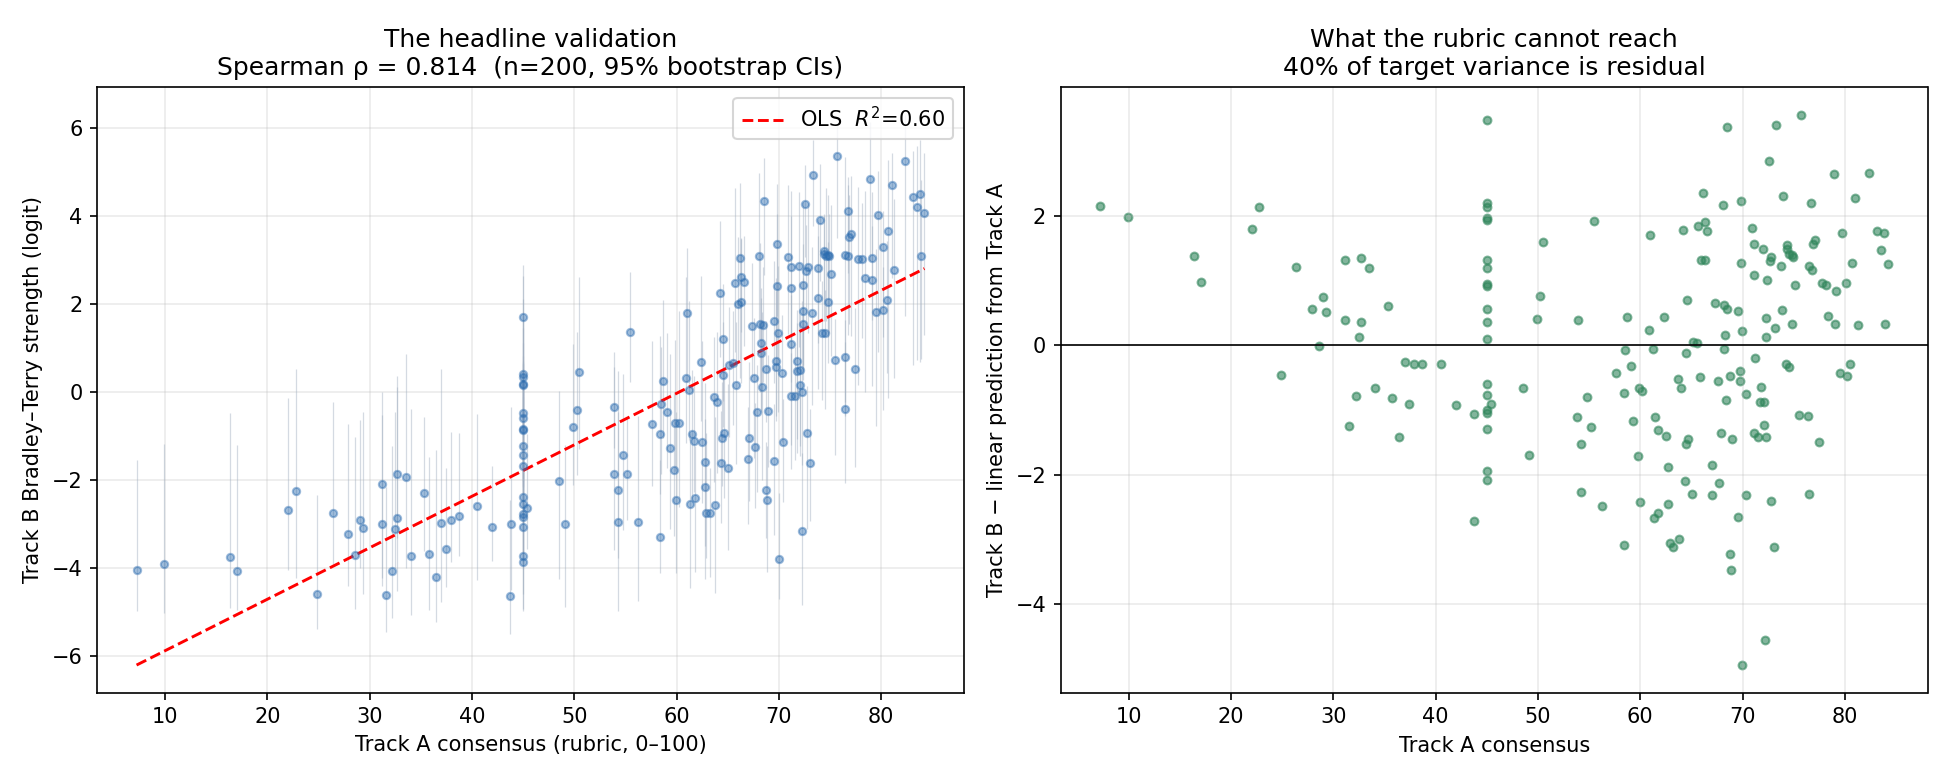
\includegraphics[width=0.92\textwidth]{figures/fig_validation.png}
\caption{Left: the learned label against the rule-based rubric. Right: where the rubric breaks
down --- accuracy on wide-gap pairs versus close pairs.}
\end{figure}

%========================================================= 6
\section{Modelling}

\subsection{Protocol}

The target is the raw Bradley--Terry logit, which is the statistically correct scale ---
unbounded and centred. The $0$--$100$ presentation score is a monotone rescaling used for
reading only and is never the training target. Of the 200 labelled universities,
\textbf{160 train / 40 test}, stratified on score band. \textbf{The test set is touched
exactly once}, in Section~6.3; no feature, hyper-parameter or threshold was chosen using it.
Model selection uses nested cross-validation (outer repeated 5-fold $\times$ 5 seeds, inner
3-fold tuning), with all imputation, scaling and selection fitted inside the training fold.

Twenty-two columns are excluded from the design matrix: identifiers, crawl metadata, the two
prestige \emph{value} columns (unusable and leaky), \texttt{load\_time\_s} and \texttt{member}
(confounded with region), and features superseded by engineered replacements. Prestige
\emph{display} flags --- does the site show a QS badge or a national rank claim --- are
retained, because ``the site advertises a badge'' is a property of the website. 78 features
remain.

\subsection{Model comparison}

\begin{table}[H]\centering\small
\caption{Nested cross-validation on the 200 labelled universities. LORO = leave-one-region-out.
The row that matters is \textbf{Track A composite}: if a transparent weighted sum matched the
learned models, the machine learning would contribute nothing and we would report that.}
\begin{tabular}{lrrrrl}
\toprule
\textbf{Model} & \textbf{CV $\rho$} & \textbf{LORO $\rho$} & \textbf{MAE} & \textbf{$R^2$} & \textbf{Verdict} \\
\midrule
LightGBM                    & 0.881 & 0.835 & 0.99 & 0.761 & beats the rubric \\
LightGBM + monotone         & 0.877 & 0.840 & 1.00 & 0.754 & beats the rubric \\
\textbf{LightGBM + label weights} & \textbf{0.873} & \textbf{0.844} & \textbf{1.00} & \textbf{0.752} & \textbf{selected} \\
RandomForest                & 0.861 & 0.825 & 1.08 & 0.705 & beats the rubric \\
Ridge                       & 0.855 & 0.830 & 1.13 & 0.687 & beats the rubric \\
\midrule
Track A composite (baseline) & 0.810 & 0.774 & 1.32 & 0.590 & --- \\
B5 content block only        & 0.752 & 0.693 & 1.39 & 0.521 & loses to the rubric \\
B9 technical block only      & 0.199 & 0.100 & 2.14 & 0.025 & loses to the rubric \\
Mean predictor               & 0.000 & 0.000 & 2.15 & $-0.001$ & loses to the rubric \\
\bottomrule
\end{tabular}
\end{table}

The selected model is \textbf{LightGBM with label weights} $w_i \propto 1/\mathrm{SE}(\beta_i)$,
so universities whose latent score was estimated confidently count for more. It is not the
best on raw cross-validation --- plain LightGBM is, at $\rho = 0.881$ --- but it is the best
under \textbf{leave-one-region-out}, which is the harder and more honest test of whether the
model learned quality rather than geography. All learned models beat the rubric with
$p < 0.001$ on a paired test across the 25 fold-repetitions.

\begin{figure}[H]\centering
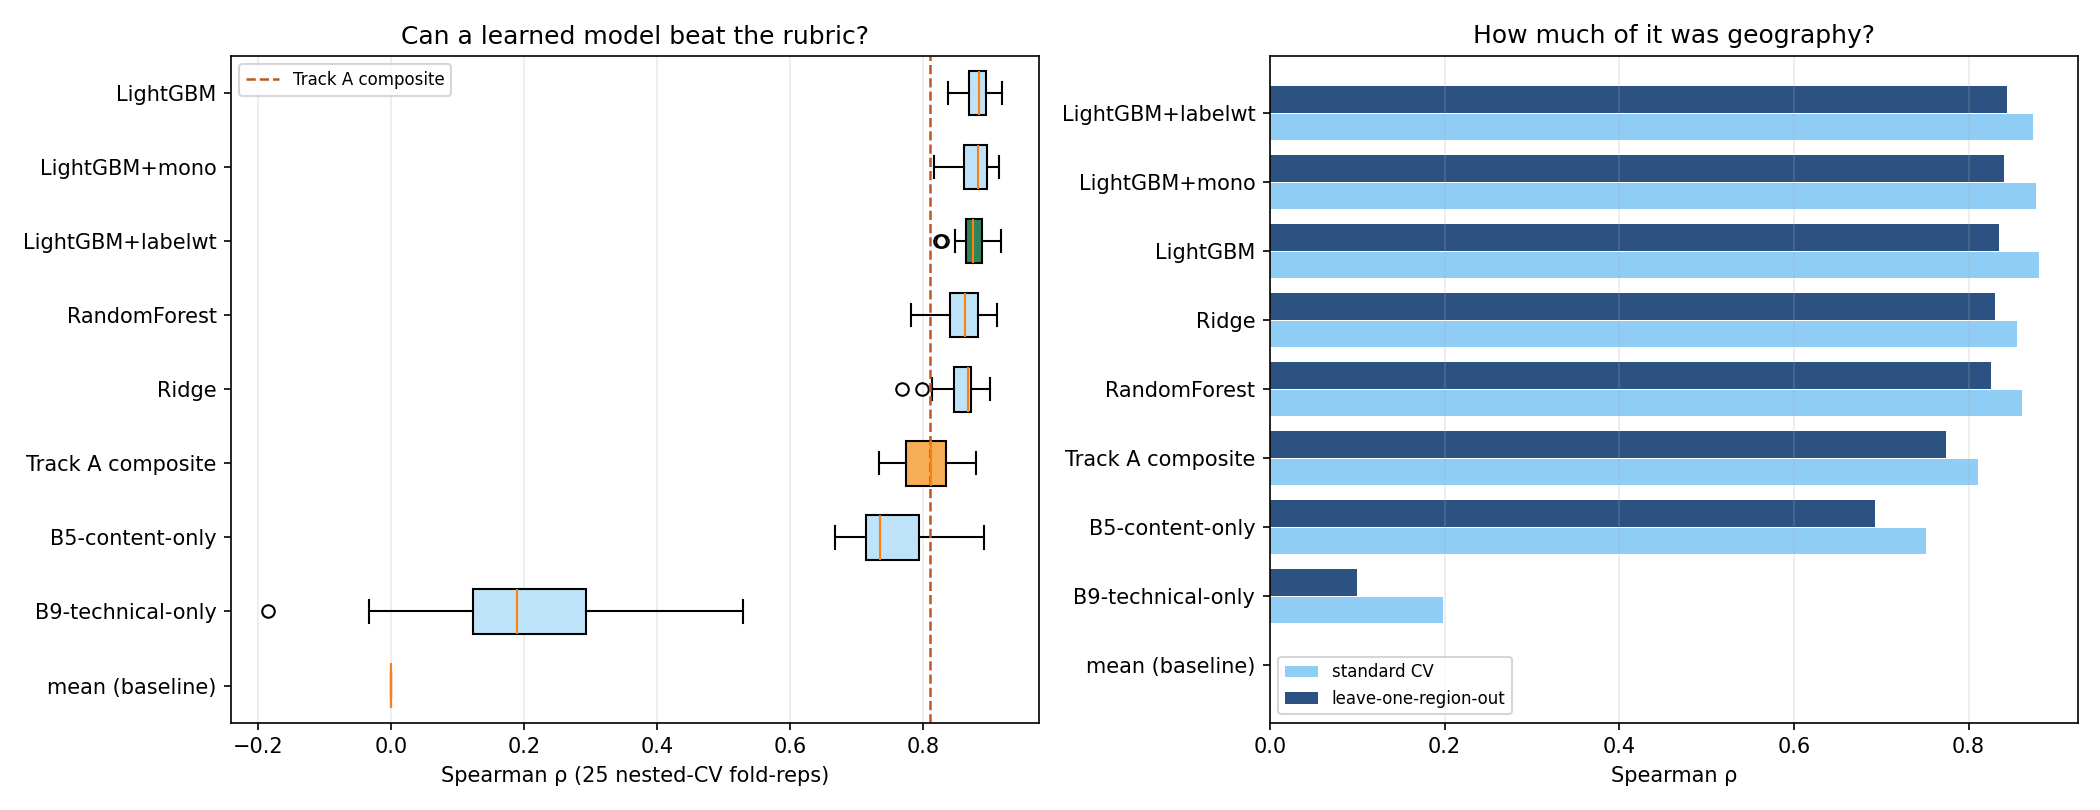
\includegraphics[width=0.92\textwidth]{figures/fig_model_comparison.png}
\caption{Model comparison. The dashed line is the transparent rubric baseline.}
\end{figure}

\subsection{Held-out test result}

\begin{table}[H]\centering
\begin{tabular}{lr}
\toprule
\multicolumn{2}{c}{\textbf{Held-out test set, $n = 40$, used once}} \\
\midrule
Spearman $\rho$ (rank agreement) & \textbf{0.922} \\
Kendall $\tau$                   & 0.736 \\
MAE (points on 0--100)           & 9.02 \\
RMSE                             & 11.44 \\
$R^2$                            & \textbf{0.818} \\
\midrule
Predictions within $\pm 10$ points & 62\% \\
Predictions within $\pm 15$ points & 78\% \\
\bottomrule
\end{tabular}
\end{table}

%========================================================= 7
\section{Results}

\subsection{The ranking}

All 1{,}226 universities are scored; the 1{,}026 without an expert label are pure inference and
were never used in fitting. Ties are broken transparently: predicted score, then content
completeness, then accessibility completeness, then \texttt{uni\_id}.

\begin{table}[H]\centering\small
\begin{minipage}[t]{0.52\textwidth}\centering
\textbf{Global top 8}\\[3pt]
\begin{tabular}{rlr}
\toprule
\# & University & Score \\
\midrule
1 & Murdoch University (AU)       & 92.2 \\
2 & University of Otago (NZ)      & 92.0 \\
3 & RWTH Aachen University (DE)   & 91.8 \\
4 & Southern Cross University (AU)& 91.7 \\
5 & University of Tartu           & 90.8 \\
6 & Polytechnic Univ.\ of Milan   & 90.5 \\
7 & University of Houston (US)    & 90.2 \\
8 & University of Porto (PT)      & 90.0 \\
\bottomrule
\end{tabular}
\end{minipage}%
\begin{minipage}[t]{0.48\textwidth}\centering
\textbf{Bangladesh top 6} (of 22)\\[3pt]
\begin{tabular}{rlrr}
\toprule
\# & University & Global & Score \\
\midrule
1 & KUET  & 31  & 85.9 \\
2 & RUET  & 66  & 81.2 \\
3 & CUET  & 86  & 79.5 \\
4 & North South Univ. & 137 & 76.7 \\
5 & Khulna University & 142 & 76.4 \\
6 & Univ.\ of Professionals & 161 & 75.7 \\
\bottomrule
\end{tabular}
\end{minipage}
\end{table}

\begin{keybox}{On KUET's position --- reported, not tuned}
KUET scores \textbf{85.9 / 100, grade A+, global rank 31, first in Bangladesh}. This is higher
than a casual visitor might expect, and we did not adjust it. The reason is visible in the
data: on the attributes this dataset actually measures, KUET's landing page ticks nearly every
box --- programmes listed, departments, faculty, library and research pages present, a notice
board posted within the last month, admission notices, scholarships, contact route, HTTPS, no
broken links, contrast 13.3:1. What the dataset \emph{cannot} see is visual design, layout
density or whether the page looks modern (Section~8). A site that satisfies every content
requirement will rank highly here even if a human would find it dated. We regard reporting
this openly as more valuable than hand-tuning the score to match intuition.
\end{keybox}

\subsection{What drives the score}

\begin{figure}[H]\centering
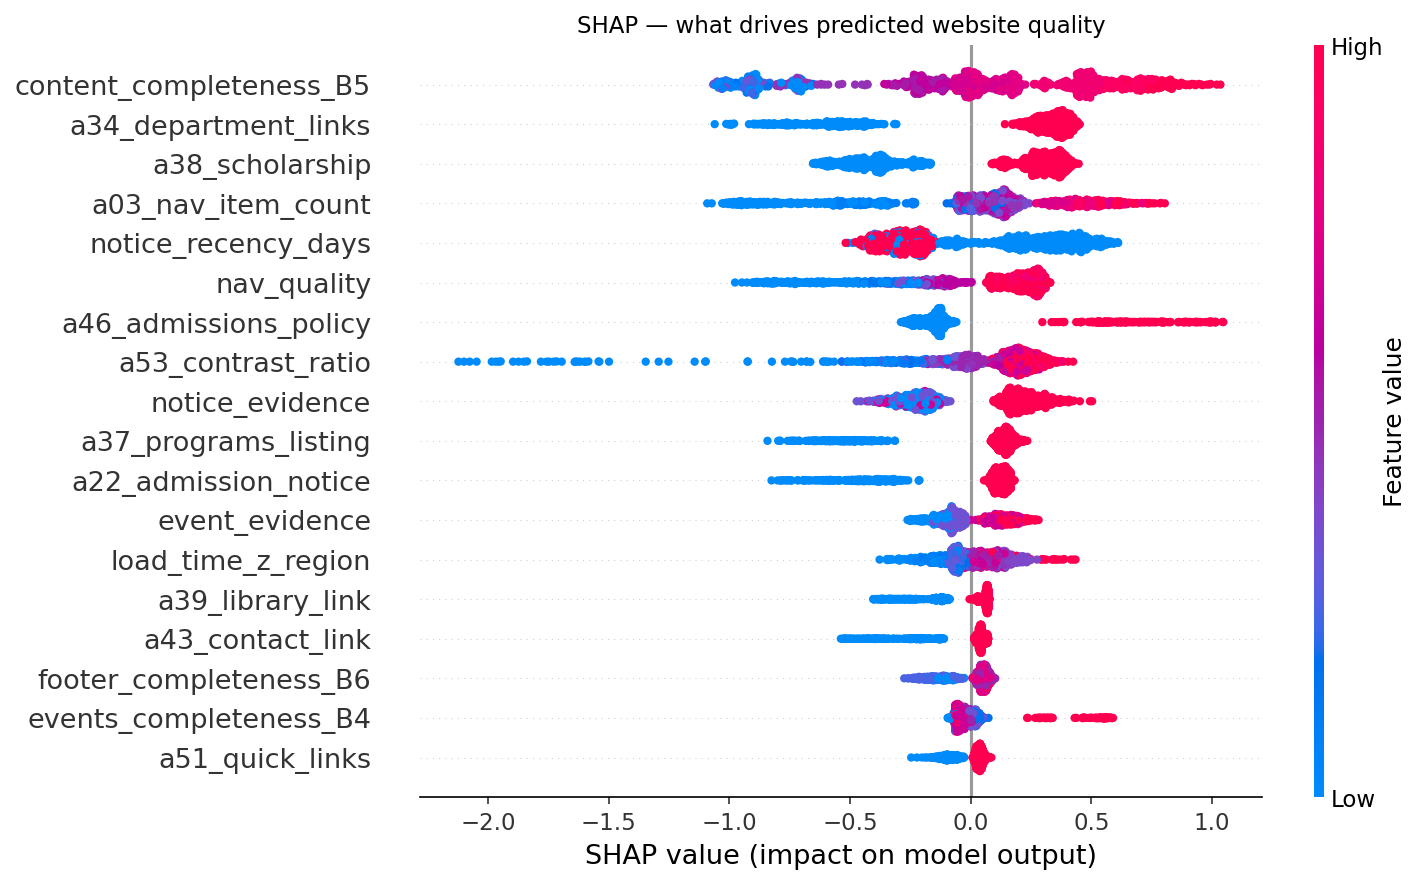
\includegraphics[width=0.88\textwidth]{figures/fig_shap.png}
\caption{SHAP values on held-out folds. The score is driven by whether the site serves a
visitor trying to apply: content completeness, department links, menu size, admissions policy,
contrast and notice recency.}
\end{figure}

\subsection{Declared weights versus realised influence}

This is the project's substantive claim about rubric design. Track~A \emph{declares} a weight
for each block; SHAP \emph{measures} the share of ranking variation each block actually drives.

\begin{table}[H]\centering\small
\caption{Declared rubric weight versus realised SHAP influence, by block.}
\begin{tabular}{lrrr}
\toprule
\textbf{Block} & \textbf{Declared \%} & \textbf{Realised \%} & \textbf{Ratio} \\
\midrule
B10 SEO metadata        & 3.6  & 0.7  & 0.18 \\
B8 service interaction  & 1.8  & 0.3  & 0.19 \\
B11 accessibility       & 6.4  & 1.3  & 0.20 \\
B6 footer               & 5.4  & 3.8  & 0.70 \\
B4 events / media       & 8.9  & 6.4  & 0.72 \\
B9 technical performance& 6.2  & 5.4  & 0.86 \\
B2 rankings / badges    & 2.1  & 2.4  & 1.12 \\
B5 page content         & 37.9 & 43.5 & 1.15 \\
B1 header / navigation  & 11.5 & 13.6 & 1.19 \\
B3 notices / updates    & 12.7 & 16.7 & 1.32 \\
B7 visual design        & 3.4  & 6.0  & 1.74 \\
\bottomrule
\end{tabular}
\end{table}

Accessibility is the sharpest case: declared at $6.4\%$, it drives $1.3\%$ --- five times less
than assigned. Under our \emph{first} label it appeared far more influential, for the reason
diagnosed in Section~4. Conversely, visual design and notice freshness both drive more than
they were given. This reproduces, on a second dataset and with a different method, the effect
Rashida et al.\ report: they allocated $40\%$ of their score to performance, which then drove
$2.9\%$ of their ranking variance, because every university scores alike on it. Hand-set
weights misallocate importance across quality dimensions, and only measuring realised
influence reveals it.

\begin{figure}[H]\centering
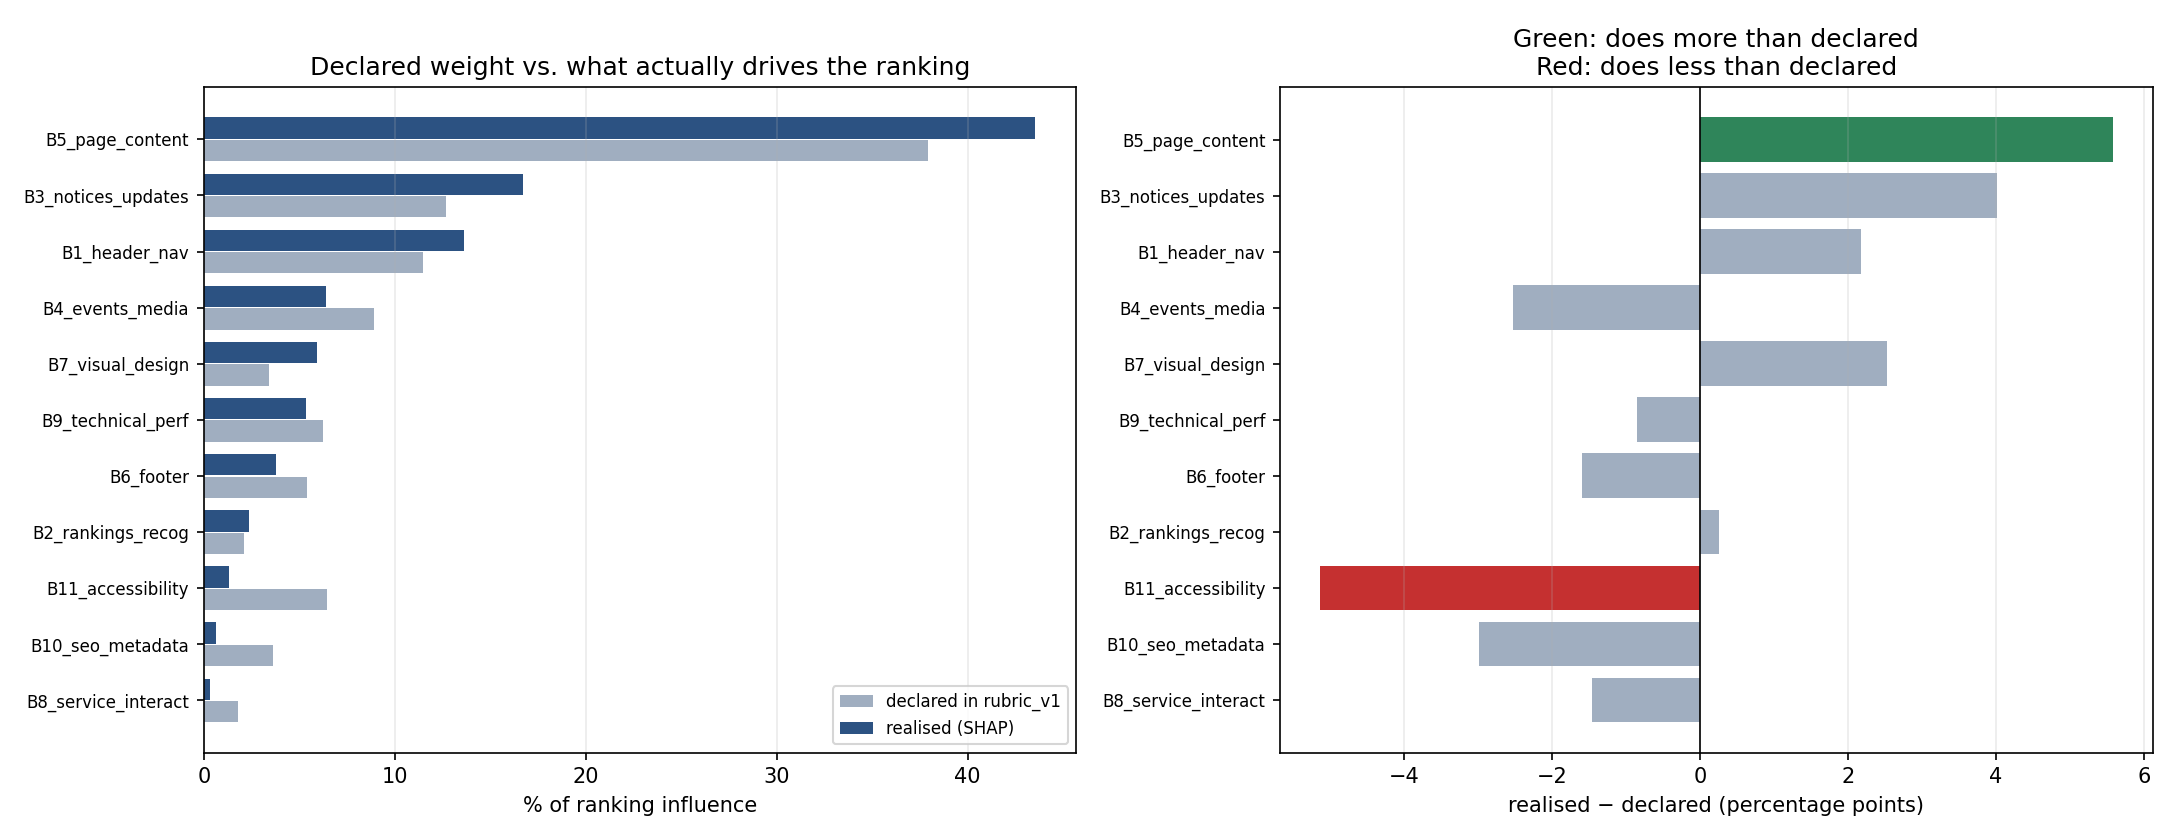
\includegraphics[width=0.88\textwidth]{figures/fig_weights.png}
\caption{Declared rubric weight against realised SHAP influence per block.}
\end{figure}

\subsection{Fairness and the collector confound}

Each of the six data collectors covered exactly one region, so \textbf{collector and geography
are perfectly confounded and cannot be separated with this data}. We therefore report model
\emph{accuracy} by region rather than claiming regional score differences are real:

\begin{center}\small
\begin{tabular}{lrrrrrr}
\toprule
Region & N.\ America & S.\ Asia+Oc. & W./N.\ Europe & E./S.\ Europe & E.\ Asia & LatAm/Africa \\
\midrule
LORO $\rho$ & 0.811 & 0.826 & 0.852 & 0.854 & 0.854 & 0.869 \\
\bottomrule
\end{tabular}
\end{center}

\noindent Accuracy is stable across all six ($0.81$--$0.87$), so the model is not a regional
lookup table. Load time is the feature most contaminated by the confound, so every ranking was
produced twice, with and without \texttt{load\_time\_z\_region}: the two orderings correlate at
$\rho = 0.992$, with a median displacement of 23 places and 264 universities moving more than
50 places. Load time therefore matters at the margin but does not determine the ranking.

\begin{figure}[H]\centering
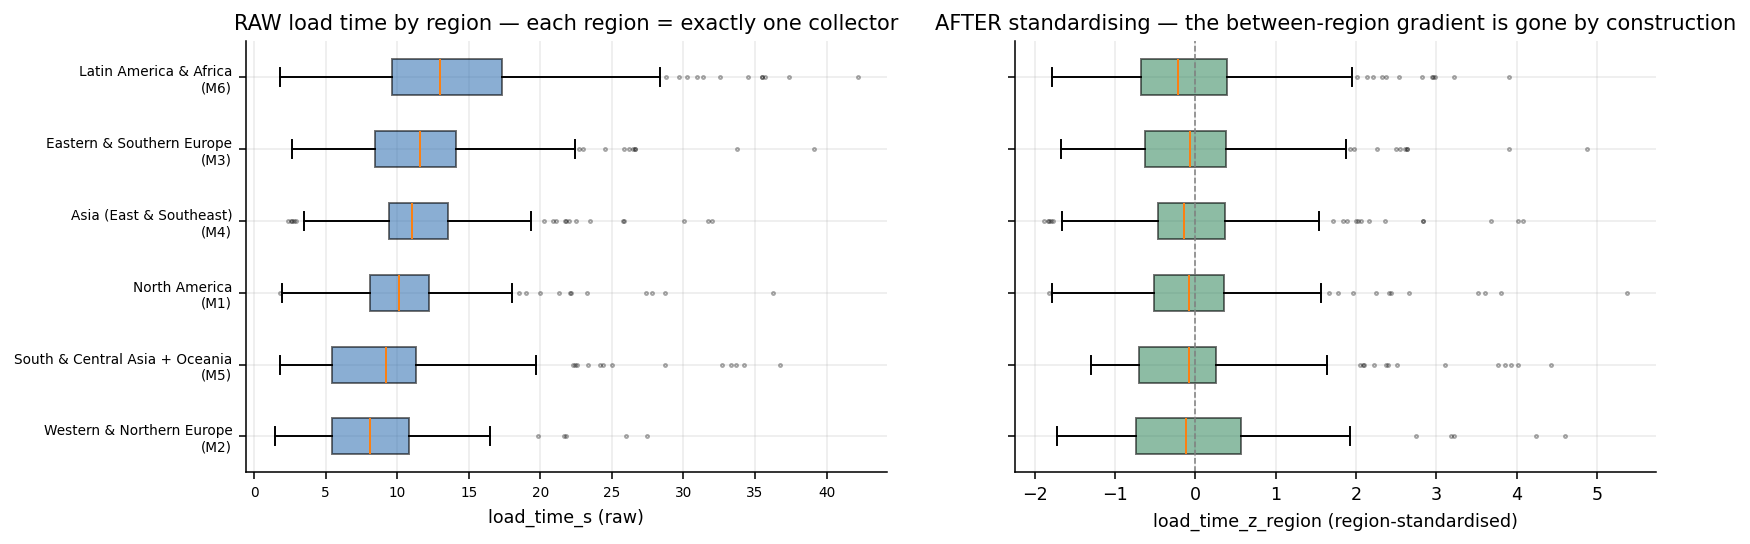
\includegraphics[width=0.85\textwidth]{figures/fig_confound.png}
\caption{Load time by collector: the confound that motivates region standardisation.}
\end{figure}

%========================================================= 8
\section{Independent Cross-Check in Weka}

The same 160/40 split was exported to ARFF and re-run with off-the-shelf Weka schemes, as an
independent check that the label is learnable and not an artefact of one library.

\begin{table}[H]\centering\small
\begin{tabular}{lrrr}
\toprule
\textbf{Weka scheme} & \textbf{Correlation} & \textbf{MAE} & \textbf{RMSE} \\
\midrule
ZeroR (baseline)      & 0.00 & 22.8 & 26.8 \\
LinearRegression      & 0.82 & 12.1 & 15.4 \\
REPTree               & 0.71 & 15.7 & 19.6 \\
RandomForest (100)    & 0.88 & 11.3 & 14.2 \\
\midrule
\emph{LightGBM (this project, Python)} & \emph{0.92} & \emph{9.0} & \emph{11.4} \\
\bottomrule
\end{tabular}
\end{table}

Weka reproduces the ranking at correlation $0.88$ with a plain random forest. A six-class
grade classifier reaches $42\%$ exact accuracy but $82\%$ within one grade --- the residual
error is boundary noise from cutting a continuous score into bands, which is precisely why the
project treats the task as regression. Full click-by-click instructions are in
\texttt{WEKA\_GUIDE.md}.

%========================================================= 9
\section{Limitations}

We state these plainly because several of them bound how the ranking should be read.

\begin{enumerate}
\item \textbf{The dataset cannot see design.} Every feature is a presence flag, a count or a
      measurement. Whether a page is cluttered, dated-looking or unpleasant to use is not in
      the 78 columns, so it cannot be in the score. This is the largest gap between this
      ranking and a real user's impression, and closing it would require screenshots and human
      raters rather than more modelling.
\item \textbf{2.0\% of rows are extraction failures, and they contaminate the bottom of the
      ranking.} 25 universities have no navigation, no programmes list, no departments page
      and no contact link recorded --- almost certainly JavaScript-rendered pages the crawler
      could not read, not genuinely empty websites. 21 of them fall in the bottom 100. The
      \emph{top} of the ranking is unaffected; the bottom should not be quoted without this
      caveat.
\item \textbf{The labels are expert-style judgments made from extracted attribute profiles},
      not ratings of live websites by a panel of humans, and must be described that way.
\item \textbf{One rater.} Self-consistency is measured ($96.7\%$ on swapped repeats);
      inter-rater agreement cannot be, because there is only one rater.
\item \textbf{No external validation} against QS, Webometrics or a student survey was
      performed, so no claim of agreement with real user perception is made.
\item \textbf{Collector and region are perfectly confounded} and this dataset cannot separate
      them. The regional ranking is the safer artefact to quote.
\item \textbf{200 labelled of 1{,}226.} The other 1{,}026 scores are model inference, flagged
      by the \texttt{has\_expert\_label} column.
\item \textbf{\texttt{a66\_broken\_links} has no denominator}, so 12 broken links on a
      20-link page and on a 2000-link page are recorded identically.
\end{enumerate}

%========================================================= 10
\section{Conclusion}

We set out to rank university websites by quality and found that the hard part was defining
quality without defining it circularly. Separating the transparent rubric (baseline) from
blind pairwise judgment (target) turns rubric--label agreement into a measurable result: they
correlate at $\rho = 0.814$, but the rubric predicts close pairs at only $62.4\%$, and it is
that residual $40\%$ of variance the model learns. On a test set used exactly once, the
selected LightGBM reaches $\rho = 0.922$ and $R^2 = 0.818$, comfortably beating the rubric at
$\rho = 0.810$, and holds $\rho = 0.844$ under leave-one-region-out.

The finding we would most want carried forward is methodological. Our first label looked
perfectly healthy by its own statistics --- $86.7\%$ self-consistent, no position bias,
correlated with the rubric at $0.790$ --- and was nonetheless measuring the wrong thing,
because the evidence we showed the judge foregrounded an attribute no visitor can perceive and
a missing-value default that inverted the meaning of freshness. No summary statistic on the
label would have caught it; reading the judge's stated reasons did. Labels deserve the same
auditing we routinely give models.

%========================================================= APPENDIX
\appendix
\section{Reproducing this work}

\begin{table}[H]\centering\small
\begin{tabular}{ll}
\toprule
\textbf{Path} & \textbf{Contents} \\
\midrule
\texttt{data/university\_websites\_labeled.csv} & all 1{,}226 universities, scored and ranked \\
\texttt{data/train.csv}, \texttt{data/test.csv} & the 160/40 expert-labelled split \\
\texttt{data/label\_provenance/} & both judgment passes, pairs, cards, fit statistics \\
\texttt{data/weka/} & the same splits as ARFF \\
\texttt{notebook/University\_Website\_Quality\_Ranking.ipynb} & the full pipeline, executed \\
\texttt{model/final\_model.joblib} & the deployed model \\
\texttt{WEKA\_GUIDE.md} & step-by-step Weka instructions \\
\bottomrule
\end{tabular}
\end{table}

\noindent The research pipeline that produced these artefacts is the nine notebooks
\texttt{01\_audit} through \texttt{09\_deliverables} in the parent project directory, which run
in order from the raw CSV with a fixed seed.

\vspace{6pt}
\noindent\textbf{Environment.} Python 3.13, pandas 2.3.3, numpy 2.4.4, scikit-learn 1.8.0,
lightgbm 4.6.0, shap 0.51.0.

\end{document}
